\documentclass{beamer}
\usepackage{ulem}
\usepackage{tikz}
\usepackage{booktabs}
\usepackage{graphicx,threeparttable,caption}
\usetikzlibrary{shapes,snakes}
\usepackage[beamer,customcolors]{hf-tikz}
\usepackage{nicematrix}
\usepackage{xcolor}
\usepackage{makecell}
\usepackage{array}
\usepackage{csquotes}
\usepackage{csquotes}
\usepackage{minted}
\captionsetup{labelformat=empty,labelsep=none}

\graphicspath{ {./png/} }

\usetikzlibrary{
    arrows,
    arrows.meta,
    shapes,
    positioning,
    shadows,
    trees,
    calc
}

\tikzset{%
    >={Latex[width=2mm,length=2mm]},
    % Specifications for style of nodes:
    plain/.style = {},
    base/.style = {
        plain,
        rectangle, rounded corners, draw=black,
        minimum width=1cm, minimum height=1cm,
        text centered, font=\sffamily\tiny\bfseries,
        fill=white, align=center
    },
    app/.style = {base, ellipse},
    data/.style = {base, fill=gray!30},
    action/.style = {base, circle, fill=red!30},
    note/.style = {app, fill=yellow},
    hl/.style={
    set fill color=red!80!black!40,
    set border color=red!80!black
    }
}


\AtBeginSection[]{
  \begin{frame}
  \vfill
  \centering
  \begin{beamercolorbox}[sep=8pt,center,shadow=true,rounded=true]{title}
    \usebeamerfont{title}\insertsectionhead\par%
  \end{beamercolorbox}
  \vfill
  \end{frame}
}
\setbeamercolor{alerted text}{fg=red}
%\usecolortheme[orchid]{structure}
\usetheme[hideothersubsections]{PaloAlto}
\makeatletter
\patchcmd{\csq@bquote@i}{{#6}}{{\emph{#6}}}{}{}
\makeatother
%\usecolortheme{orchid}
%\usefonttheme{professionalfonts}
\newcommand{\soutthick}[1]{%
   \textcolor{red}{
   \renewcommand{\ULthickness}{1pt}%
      \sout{#1}%
   \renewcommand{\ULthickness}{.4pt}% Resetting to ulem default
   }
}
\newcommand{\centered}[1]{\begin{tabular}{l} #1 \end{tabular}}
\setbeamertemplate{section in toc}[square]
\setbeamertemplate{subsection in toc}[square]
\setbeamertemplate{section in sidebar}[shaded]
\setbeamertemplate{items}[square]
\setbeamercovered{transparent} 

\title[]{Introduction to Computational Social Science}
\subtitle{Computer simulation -- why simulate?}
\author[]{Mikołaj Biesaga\\ \small{\color{blue}{\href{mailto:m.biesaga@uw.edu.pl}{m.biesaga@uw.edu.pl}}}}
\institute{
\includegraphics[width = 4 cm]{uw.png}}
\date{April 8, 2025}
\begin{document}
\begin{frame}
   \titlepage
\end{frame}

\begin{frame}
   \frametitle{What is a model?}
   \only<1>{
      \begin{figure}
         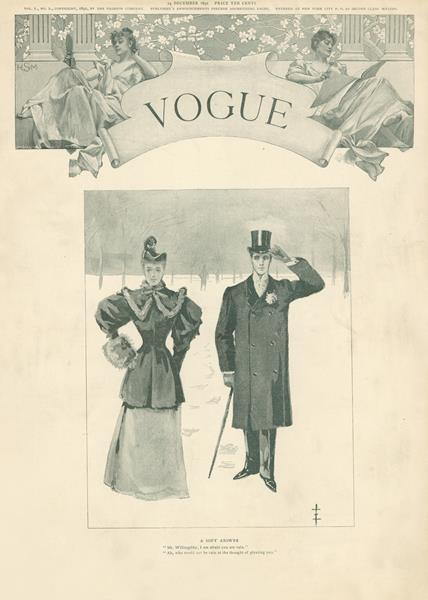
\includegraphics[width = .48\textwidth]{vogue.jpg}
         \caption{from \href{https://archive.vogue.com/issue/18921224}{\textcolor{blue}{Vogue}} (December 24, 1892)}

      \end{figure}
   }
   \only<2>{
      \begin{block}{Model}
         In simple terms a model is a \underline{simplified} representation of a system (reality) that helps to understand how the system works/worked in the past/will work in the future.
      \end{block}
   }
   \only<3,4>{
      \begin{itemize}
         \item What is a model? \href{https://youtu.be/RK9m4OmFAbY?feature=shared}{\textcolor{blue}{YouTueb video}}
         \item<4> Formalizing a theory into a model allows the researcher to
         describe their ideas in a precise, unambiguous way (Goldstone \& Janssen 2005; Epstein 2008). 
         \item<4> Models are conceptually precise, their assumptions are clear;
         they allow formal deduction and an easy way to verify their internal
         validity (Timpone \& Taber 1996). 
         \item<4> Last but not least they provide an unambiguous way to
         communicate within the scientific community (Nowak, Rychwalska, \&
         Borkowski, 2015).
      \end{itemize}
      %% \begin{itemize}
      %%    \item What is a model? \href{https://www.youtube.com/watch?v=uWuNfhDvZz8}{\textcolor{blue}{YouTube video}}
      %% \end{itemize}
   }
   \only<5>{
      \framesubtitle{Simulating}
      \begin{tikzpicture}
         \node [text width = 1.5cm] at (0,0) {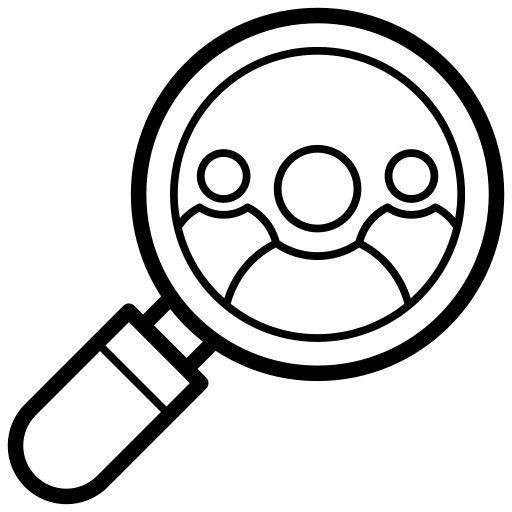
\includegraphics[width = \textwidth]{observation.png}};
         \node at (0,-2) {\footnotesize\textsc{Observation}};
         \node [text width = 1.5cm] at (2.5,0) {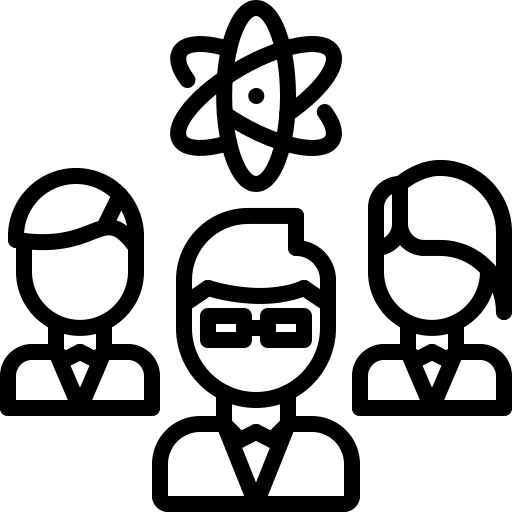
\includegraphics[width = \textwidth]{theory_formulation.png}};
         \node [text width = 2cm, align = center] at (2.5,-2) {\footnotesize\textsc{Theory \\Formulation}};
         \node [text width = 1.5cm] at (5,0) {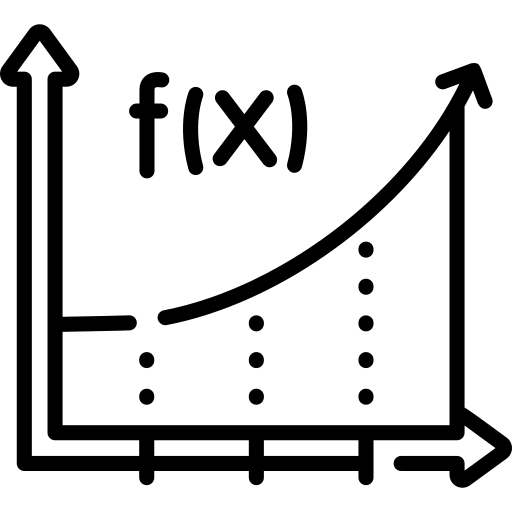
\includegraphics[width = \textwidth]{modeling.png}};
         \node [text width = 1.5cm, align = center] at (5,-2) {\footnotesize\textsc{Model \\Creation}};
         \node [text width = 1.5cm] at (7.5,0) {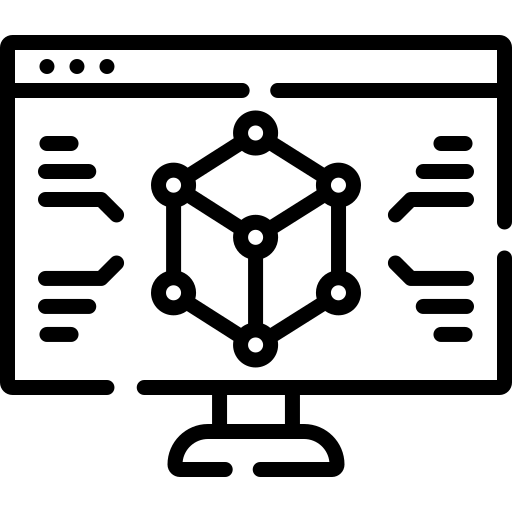
\includegraphics[width = \textwidth]{simulation.png}};
         \node at (7.5,-2) {\footnotesize\textsc{Simulating}};
         \draw [thick, ->] (.8,0) -- (1.7,0);
         \draw [thick, ->] (3.3,0) -- (4.2,0);
         \draw [thick, ->] (5.8,0) -- (6.7,0);
      \end{tikzpicture}
   }

\end{frame}

\begin{frame}
   \frametitle{Why simulate?}
   \framesubtitle{Nowak, Rychwalska, \& Borkowski, 2015}
   \begin{enumerate}
      \item What is a mental model?
         \begin{itemize}
            \item "Mental models are the mind's replicas of phenomena, upon
            which humans manipulate to learn the mechanism and workings of the
            surrounding environment." (Ibidem, p.~2)
            \item Mental models develop most accurately through interaction with
            the target system (Norman, 1983).
         \end{itemize}
      \item What are the benefits of simulating for scientists?
   \end{enumerate}
\end{frame}

\begin{frame}
   \frametitle{What are computer simulations?}
   \only<1>{
      \begin{block}{Computer Simulation}
         Computer simulation is the running of a model on a computer, the model
         being designed to represent the behaviour of, or the outcome of, a
         real-world or physical system. The reliability of some models
         can be determined by comparing their results to the real-world outcomes
         they aim to predict/explain.
      \end{block}
   }
   \only<2>{
      \framesubtitle{How are they useful?}

   }
   \only<3>{
      \framesubtitle{Agent-based models}
      \begin{itemize}
         \item 

      \end{itemize}

   }
   \only<4>{
      \framesubtitle{Monte-Carlo Simulations}

   }

\end{frame}

\begin{frame}
   \frametitle{Dynamic models of segregation}
   \framesubtitle{Schelling, 1971}

\end{frame}

\begin{frame}
   \frametitle{The world of polygons}
   \begin{figure}
      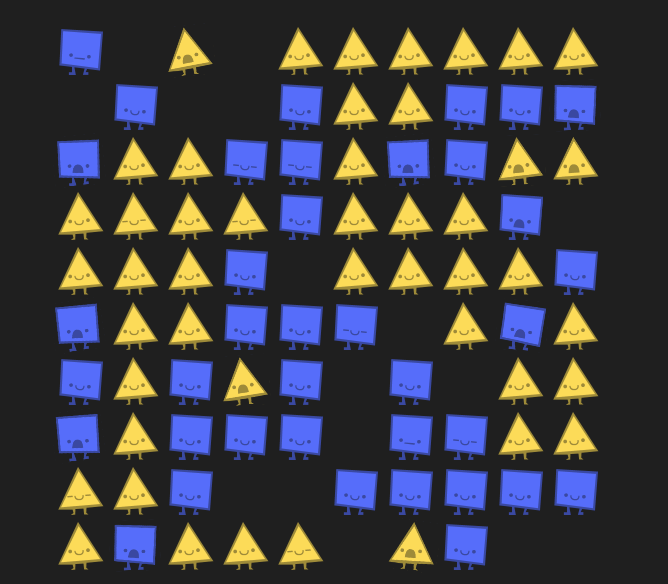
\includegraphics[width = .7\textwidth]{polygons.png}
      \caption{by Nicky Case from \href{https://ncase.me/polygons/}{\textcolor{blue}{https://ncase.me/polygons/}}}
   \end{figure}

\end{frame}

\begin{frame}
   \frametitle{Modeling Dynamics of Multicultural Integration and Conflict}
   \framesubtitle{de Raad, Nowak, \& Borkowski, 2013}

\end{frame}

\end{document}